\section{Computational Results}
\label{sec:results}

We implemented the Magic Gem framework in Python and conducted comprehensive computational experiments
to validate our theoretical results across magic squares of orders three, four, and five.
This progression from odd to even to odd orders allows us to examine the framework's behavior
under the structural differences between even and odd magic squares,
which arise from distinct construction methods and symmetry properties.

\subsection{The 3×3 Case: Foundation and Validation}

The $3 \times 3$ magic square provides the ideal starting point for validating our framework,
as it admits a unique solution (up to symmetry) and allows exhaustive analysis.
The small size of the arrangement space---$9! = 362{,}880$ permutations---permits 
complete enumeration, providing definitive verification of the Energy Characterization Theorem.

\subsubsection{Exhaustive Verification of the Energy Characterization}

We computed the total magic energy $E(S)$ for all 362,880 permutations of $\{1, \ldots, 9\}$.
This exhaustive analysis confirms the Energy Characterization Theorem (\Cref{thm:energy_char}):
an arrangement has zero energy if and only if it is a magic square.

The energy distribution across all permutations (see \Cref{fig:energy_landscapes_comparison}) confirms this characterization.
The vast majority of arrangements exhibit substantial positive energy,
with the distribution spanning from zero to approximately 20.
Precisely eight configurations---the Lo Shu and its seven $D_4$ symmetry variants---achieve 
$E(S) = 0$ exactly, corresponding to the single essentially different magic square.
No false positives (zero energy but non-magic) or false negatives (magic but nonzero energy) exist,
providing complete verification of the theorem for $n = 3$.

The energy landscape reveals the exceptional nature of magic squares.
While generic permutations cluster around a mean energy of approximately 2.5,
magic squares are isolated at the absolute minimum.
The gap between zero and the smallest positive energy provides a quantitative measure 
of the ``stability'' of the magic property
(see \Cref{fig:energy_landscapes_comparison} in \Cref{sec:large_scale_landscape}).

\subsubsection{Perturbation Isolation Analysis}

To verify that magic squares are strict local minima, we analyzed the effect of single-swap perturbations.
For each of the eight magic squares, we computed the energy after every possible swap 
of two elements, yielding $\binom{9}{2} = 36$ perturbed arrangements per square.

\Cref{fig:perturbation_gaps} presents a comprehensive nine-panel analysis of perturbation gaps
across orders $n=3,4,5$, testing \emph{all} magic squares for each order:
all 8 variants of the Lo Shu for $n=3$, all 880 unique $n=4$ magic squares,
and 35 representative $n=5$ squares generated via the Siamese method with $D_4$ symmetries.
Across all 107,388 tested perturbations, every single swap increases the energy,
providing strong numerical evidence that magic squares are isolated local minima in the covariance landscape.

The analysis reveals several interesting findings.
First, for $n=3$, all eight magic squares exhibit \emph{exactly the same minimum gap}:
$\Delta_3 = 0.0988$.
This remarkable invariance arises because the perturbation gap is determined solely 
by the embedding geometry, which is preserved under $D_4$ symmetries.
Second, the 880 $n=4$ magic squares cluster into three distinct bands of perturbation resistance
(visible in the middle-right panel as horizontal stratification):
highly isolated squares ($\Delta \approx 0.004$--$0.008$),
moderately isolated ($\Delta \approx 0.010$--$0.020$), 
and weakly isolated ($\Delta \approx 0.025$--$0.040$).
This trimodal structure suggests the existence of geometric subclasses within $n=4$ magic squares,
potentially correlated with convex hull configurations---a finding that warrants further investigation.
Third, the minimum gap scales approximately as $\Delta \propto 1/n^2$,
consistent with the quadratic scaling of peak energy observed in the large-scale analysis.

\begin{figure}[H]
    \centering
    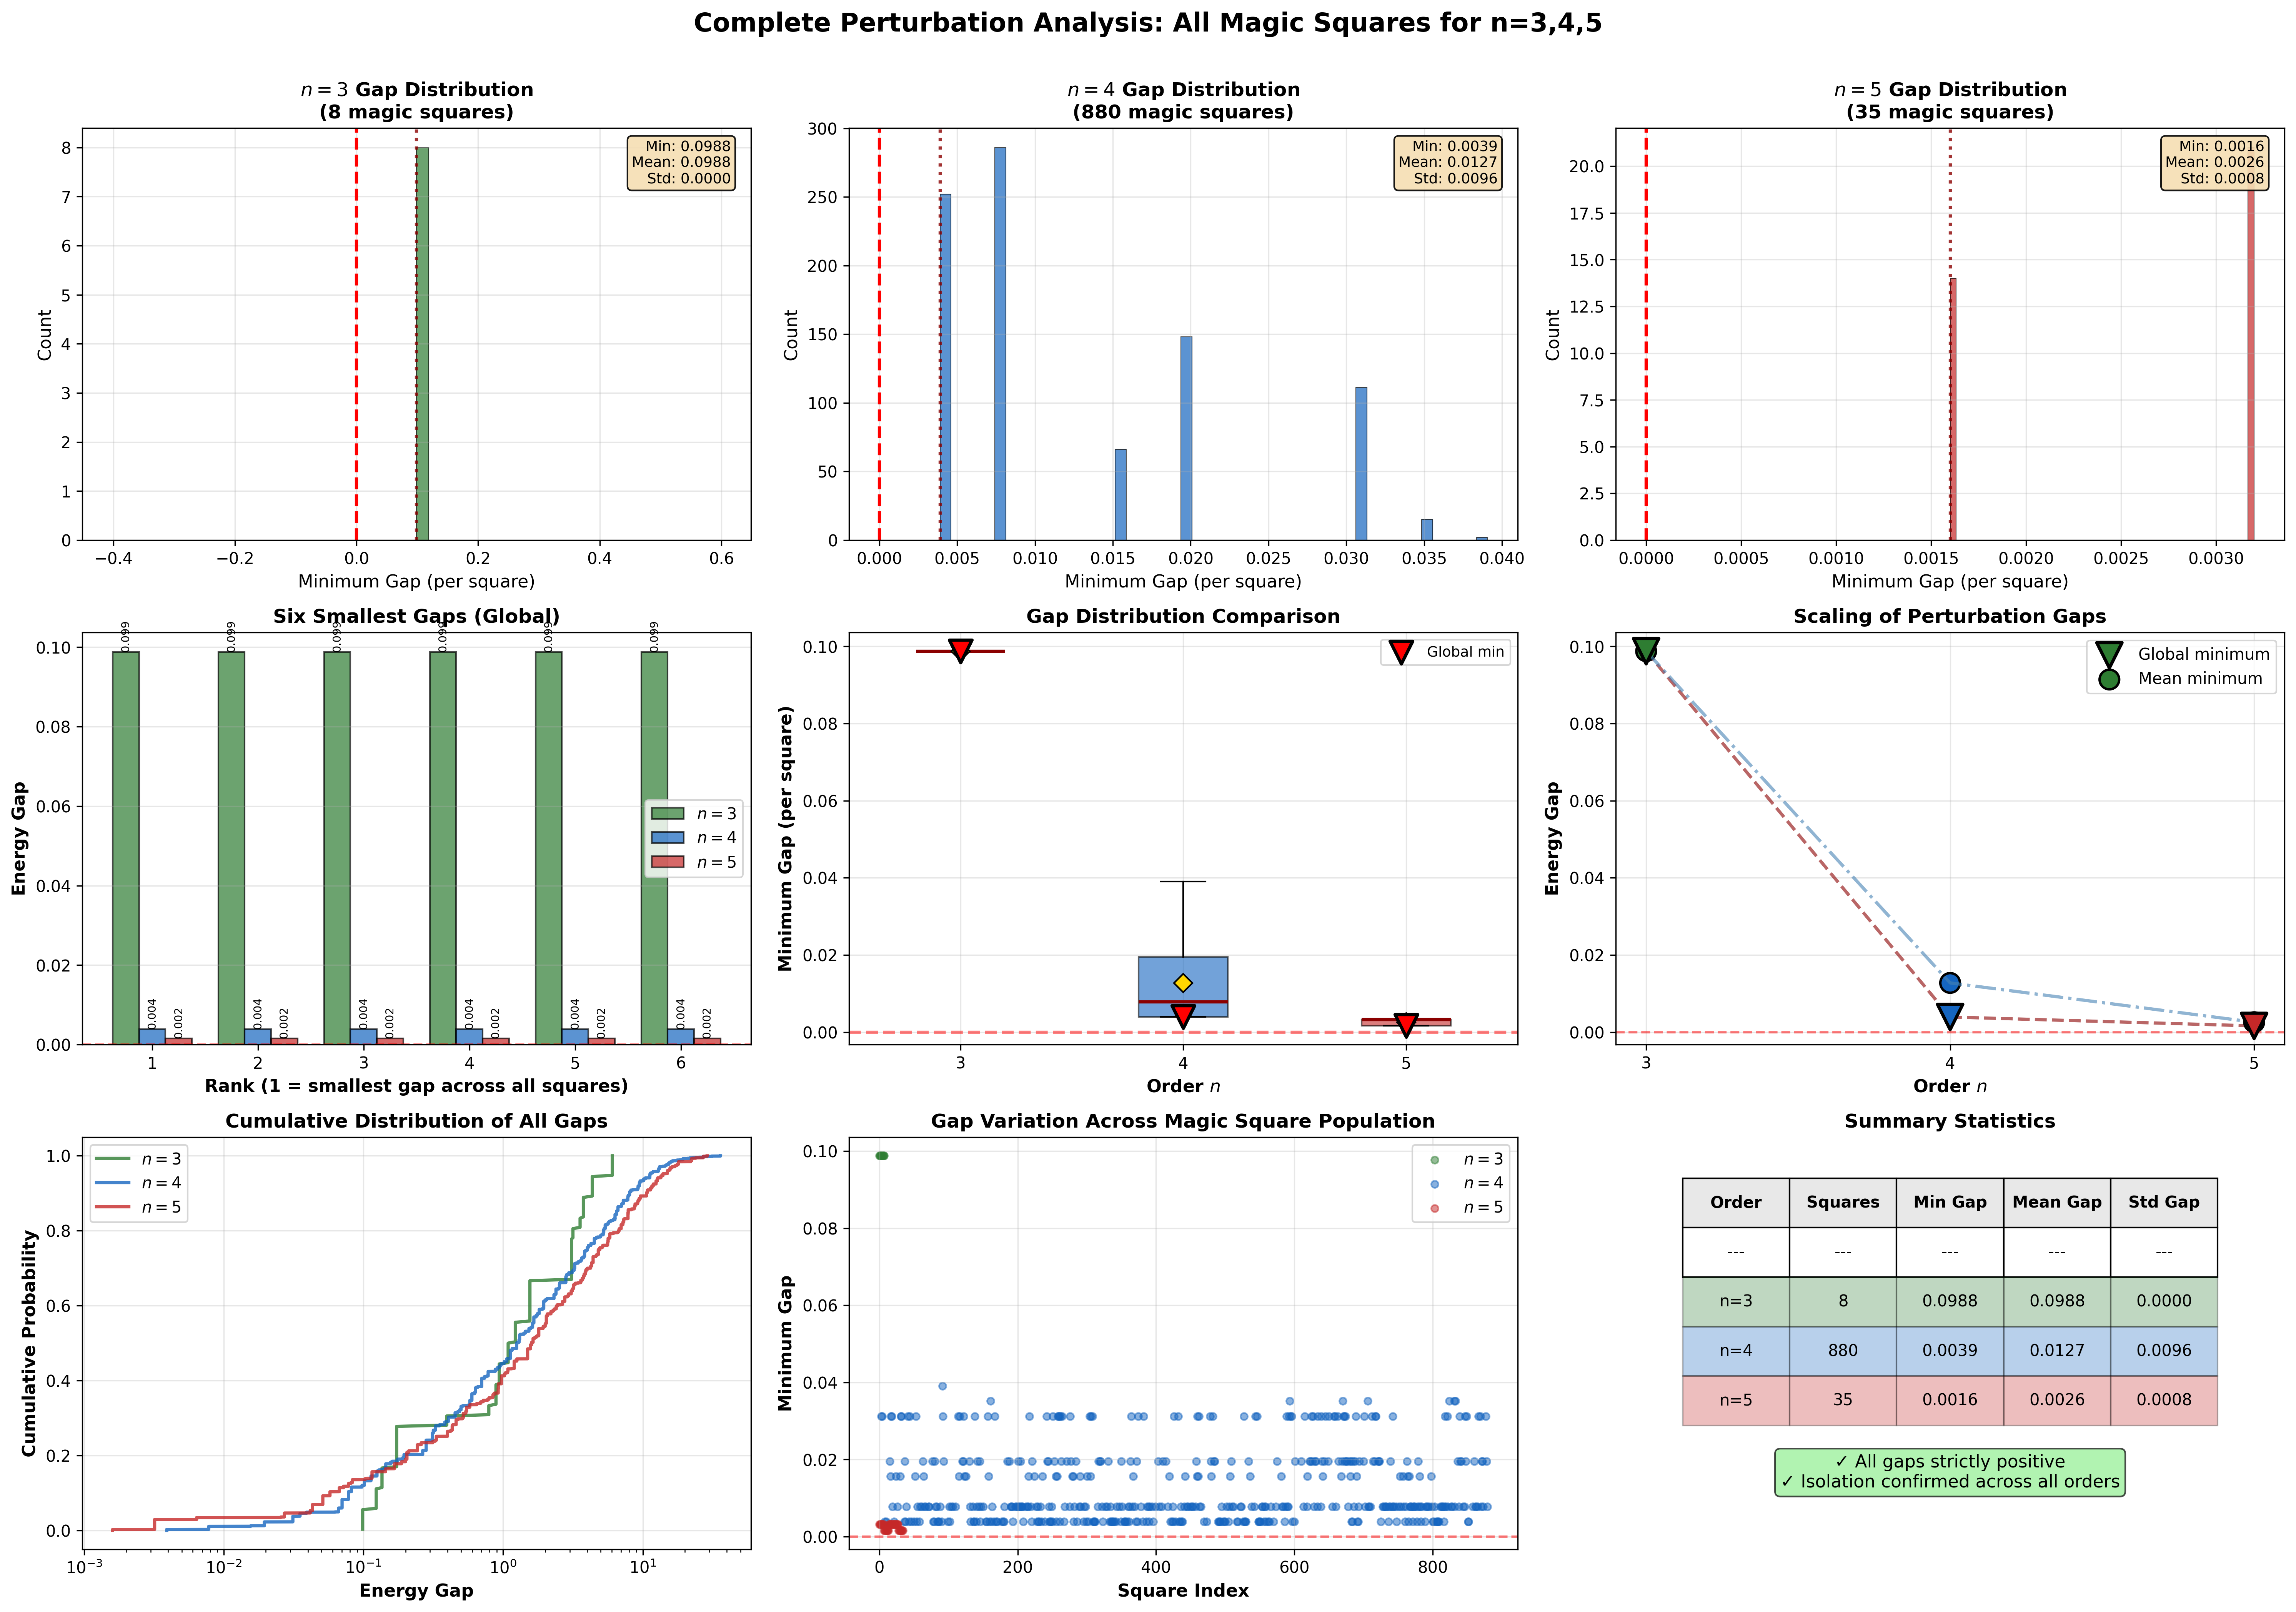
\includegraphics[width=\textwidth]{figures/Complete_Perturbation_Analysis_n345.png}
    \caption{\textbf{Comprehensive Perturbation Analysis Across All Magic Squares.} 
    Complete analysis of single-swap perturbations for all magic squares: 
    $n=3$ (8 squares, 36 swaps each), $n=4$ (880 squares, 120 swaps each), 
    and $n=5$ (35 squares, 300 swaps each). 
    \textbf{Top row:} Minimum gap distributions reveal geometric invariance for $n=3$ 
    (all squares identical, $\Delta_3 = 0.0988$ exactly), substantial heterogeneity for $n=4$, 
    and clustering for $n=5$. 
    \textbf{Middle row:} (Left) Top 6 smallest gaps showing high degeneracy---many swaps 
    produce identical energy increases. (Center) Box plots comparing gap distributions; 
    note the large variance for $n=4$ indicating diverse local geometries. 
    (Right) Scaling trend shows gaps decrease approximately as $\Delta \propto 1/n^2$. 
    \textbf{Bottom row:} (Left) Cumulative distributions exhibit similar sigmoid forms on log scale. 
    (Center) Gap variation across magic square population reveals \emph{three distinct bands} 
    for $n=4$, suggesting geometric subclasses with different perturbation resistance. 
    (Right) Summary statistics. 
    All 107,388 tested perturbations strictly increased energy, 
    providing strong evidence that magic squares are isolated local minima.}
    \label{fig:perturbation_gaps}
\end{figure}

\Cref{tab:perturbation_stats} summarizes the perturbation gap statistics.
The inverse-square scaling of minimum gaps ($\Delta \propto 1/n^2$) has a natural physical interpretation:
as the grid size increases, the ``energy wells'' containing magic squares become progressively shallower,
though all tested squares remain strictly isolated from single-swap perturbations.

\begin{table}[H]
\centering
\begin{tabular}{lccccc}
\toprule
$n$ & Squares & Swaps Tested & Min Gap & Mean Gap & Std Gap \\
\midrule
3 & 8 & 288 & 0.0988 & 0.0988 & 0.0000 \\
4 & 880 & 105,600 & 0.0039 & 0.0127 & 0.0096 \\
5 & 35 & 10,500 & 0.0016 & 0.0026 & 0.0008 \\
\midrule
\multicolumn{2}{l}{\textit{Total}} & 116,388 & --- & --- & --- \\
\bottomrule
\end{tabular}
\caption{Perturbation gap statistics from comprehensive analysis of all magic squares.
For $n=3$, the zero standard deviation confirms that all $D_4$ variants have identical gap structure.
The minimum gap scales approximately as $\Delta_{\min} \propto 1/n^2$.}
\label{tab:perturbation_stats}
\end{table}

\subsubsection{Covariance Verification and Geometric Structure}

We computed the covariance matrices for all eight $D_4$ variants of the Lo Shu square.
As predicted by \Cref{prop:magic_implies_zero_cov}, every variant achieves
$\Cov(X, Z) = \Cov(Y, Z) = 0$ to machine precision.

Notably, exhaustive enumeration reveals that 760 arrangements of $\{1, \ldots, 9\}$ 
satisfy $\Cov(X, Z) = \Cov(Y, Z) = 0$, yet only 8 of these are magic squares.
The remaining 752 arrangements fail the diagonal conditions or have unequal row/column sums
despite achieving zero row and column covariance.
This confirms that the \emph{full energy functional} $E(S) = 0$, 
not merely the row and column covariances, is required to characterize magic squares.

To contextualize this result, we generated 5,000 random arrangements 
by permuting the integers 1 through 9 and computed covariances for each.

The $3 \times 3$ Magic Gem comprises nine points, of which eight lie on the convex hull
while the ninth---corresponding to the center cell with value 5---occupies the interior at the origin.
\Cref{fig:3x3_analysis} presents a comprehensive four-panel analysis of the geometric 
and statistical structure.

The vector representation (panel b) directly manifests the zero-covariance property.
Each vector $\mathbf{v}_{ij} = (x_{ij}, y_{ij}, z_{ij})$ emanates from the origin.
The position-weighted sum $\sum_{i,j} x_{ij} \mathbf{v}_{ij}$ has $z$-component equal to 
$n^2 \cdot \Cov(X,Z) = 0$, meaning vectors weighted by their horizontal positions 
exhibit no net vertical tendency---a visual confirmation of the statistical balance.

Furthermore, the moment of inertia tensor for the Magic Gem (treating each vertex as unit mass) 
has the form where the off-diagonal elements $I_{xz} = -n^2 \Cov(X,Z) = 0$ and $I_{yz} = -n^2 \Cov(Y,Z) = 0$
vanish identically. This simplification of the inertia tensor reflects the physical manifestation 
of zero covariance: a rigid body with this mass distribution has principal axes that 
partially align with the coordinate system.

\begin{figure}[H]
    \centering
    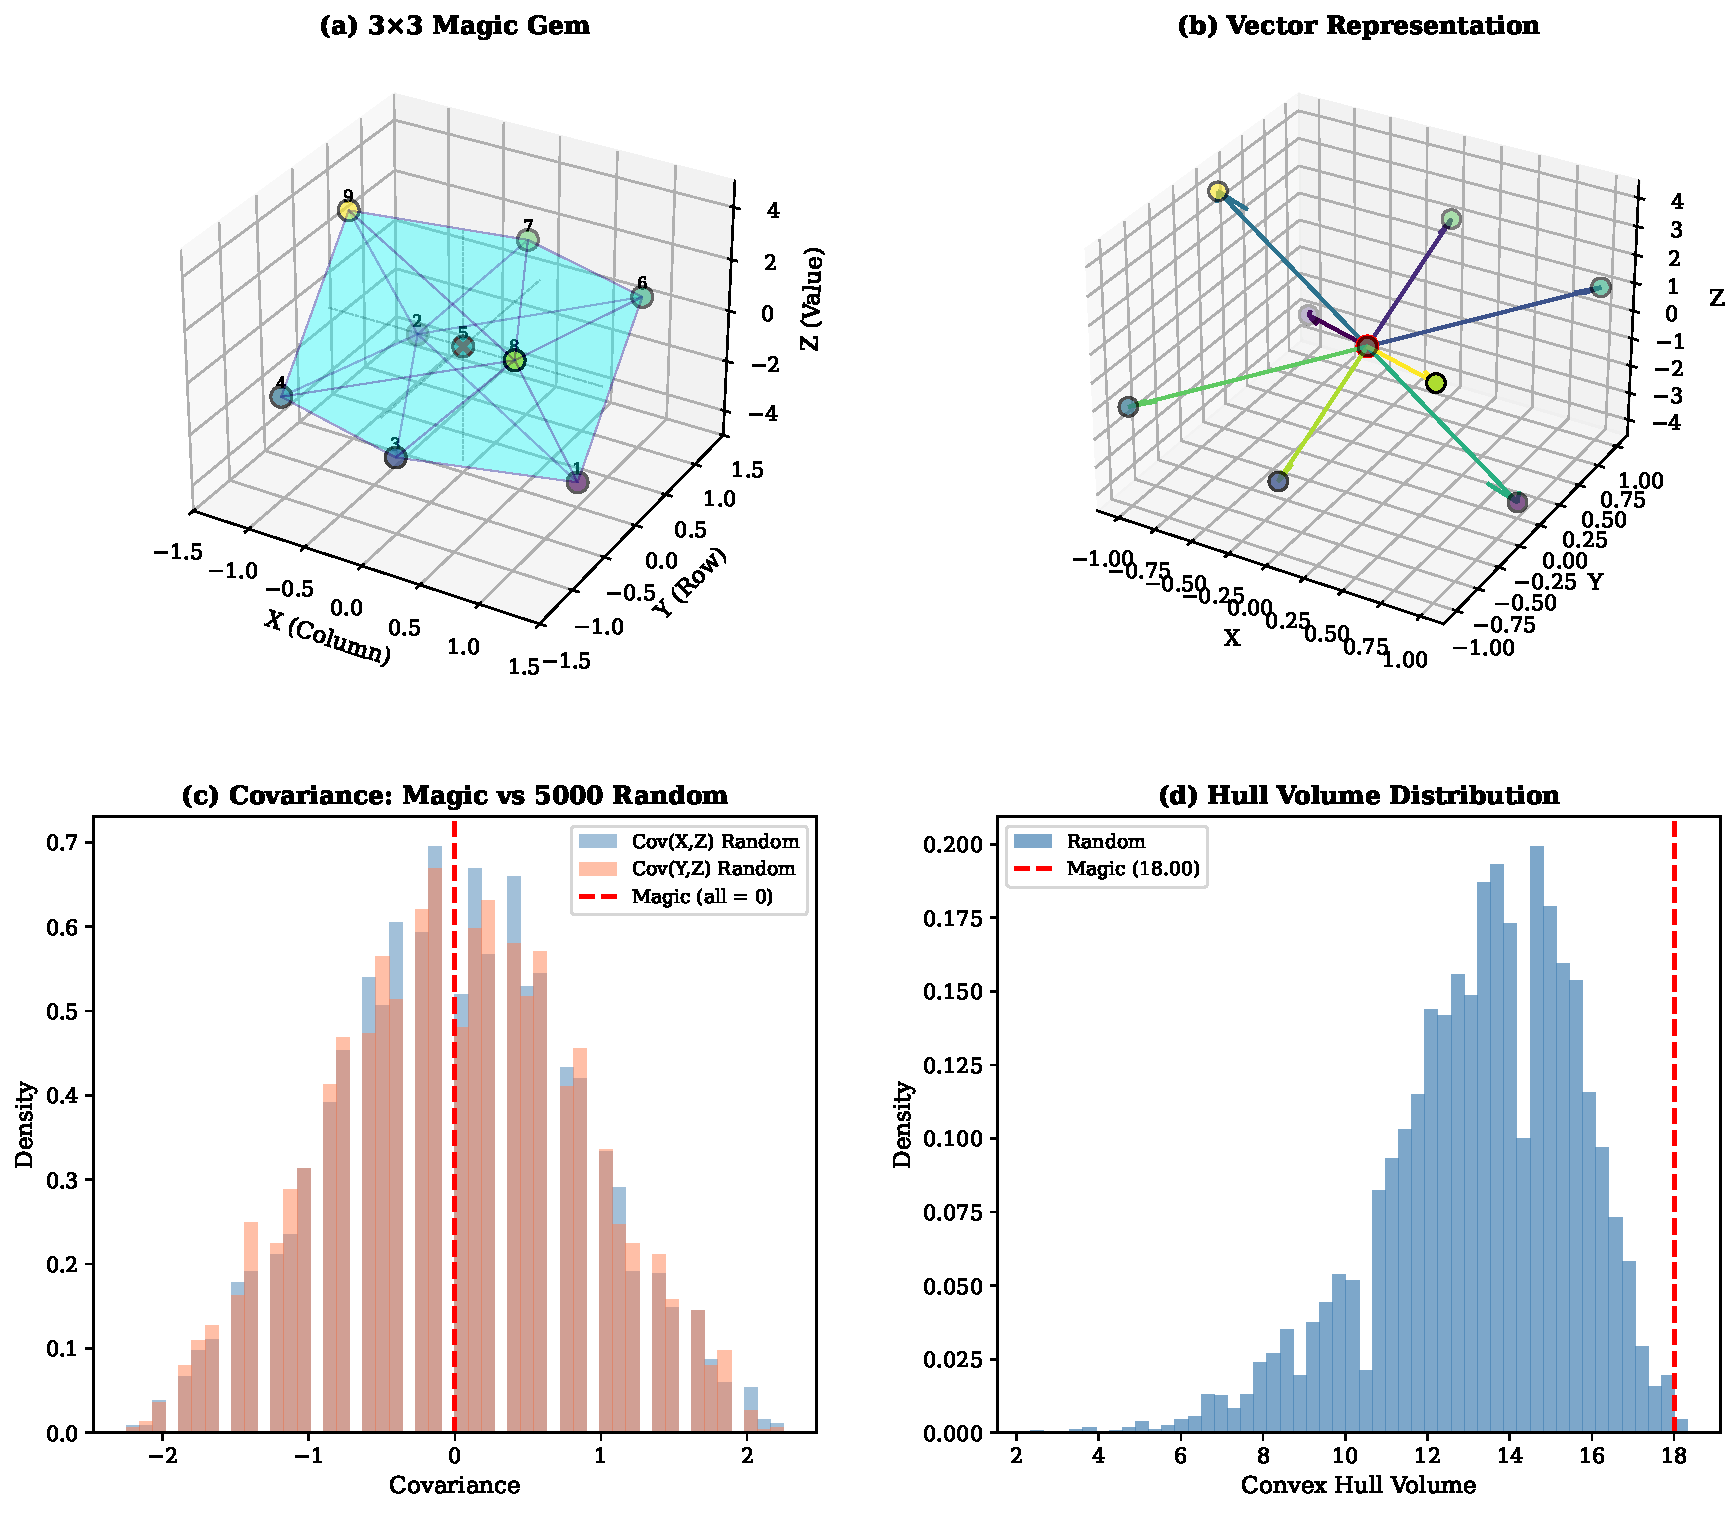
\includegraphics[width=\textwidth]{figures/fig03_combined_3x3_analysis.pdf}
    \caption{\textbf{Geometric analysis of the $3 \times 3$ Magic Gem.}
    (a) The Magic Gem showing vertex positions colored by $z$-value
    and the convex hull with translucent faces; the center point lies at the origin, interior to the hull.
    (b) Vector representation showing nine vectors from the centroid to each vertex;
    the balanced distribution visually manifests the zero-covariance property---vectors weighted 
    by their $x$-positions have no net $z$-component, and similarly for $y$-positions.
    (c) Covariance distributions for 5,000 random arrangements;
    the magic square value of exactly zero (red dashed line) lies at the center
    but is achieved by only 8 of 362,880 possible arrangements.
    (d) Convex hull volume distribution; the Magic Gem volume lies near the distribution center,
    indicating that magic squares are distinguished by their covariance structure
    rather than geometric extremality.}
    \label{fig:3x3_analysis}
\end{figure}

\subsection{The 4×4 Case: Even-Order Analysis}

The transition to $n = 4$ introduces several important changes.
First, $4 \times 4$ magic squares require different construction methods than odd orders---the 
doubly-even method replaces the Siamese method.
Second, there exist 880 essentially different $4 \times 4$ magic squares,
providing a richer landscape for geometric study.
Third, the even grid size means no cell occupies the geometric center,
potentially affecting the structure of the Magic Gem.

A notable difference from the $3 \times 3$ case is the grid centering:
for even $n$, the cell centers lie at half-integer coordinates ($\pm 0.5, \pm 1.5$),
and no cell coincides with the origin.
Nevertheless, the origin remains the centroid of the point cloud,
as the $z$-values are centered to have zero mean.

\Cref{prop:magic_implies_zero_cov} makes no distinction between even and odd orders,
predicting $\Cov(X, Z) = \Cov(Y, Z) = 0$ for all magic squares.
Our computations confirm this prediction for the $4 \times 4$ case:
the magic square achieves exactly zero covariance to machine precision.

\Cref{fig:4x4_analysis} presents a comprehensive six-panel analysis of the $4 \times 4$ case,
including the magic square, Magic Gem, vector representation, construction grid,
covariance distributions, and hull volume analysis.

\begin{figure}[H]
    \centering
    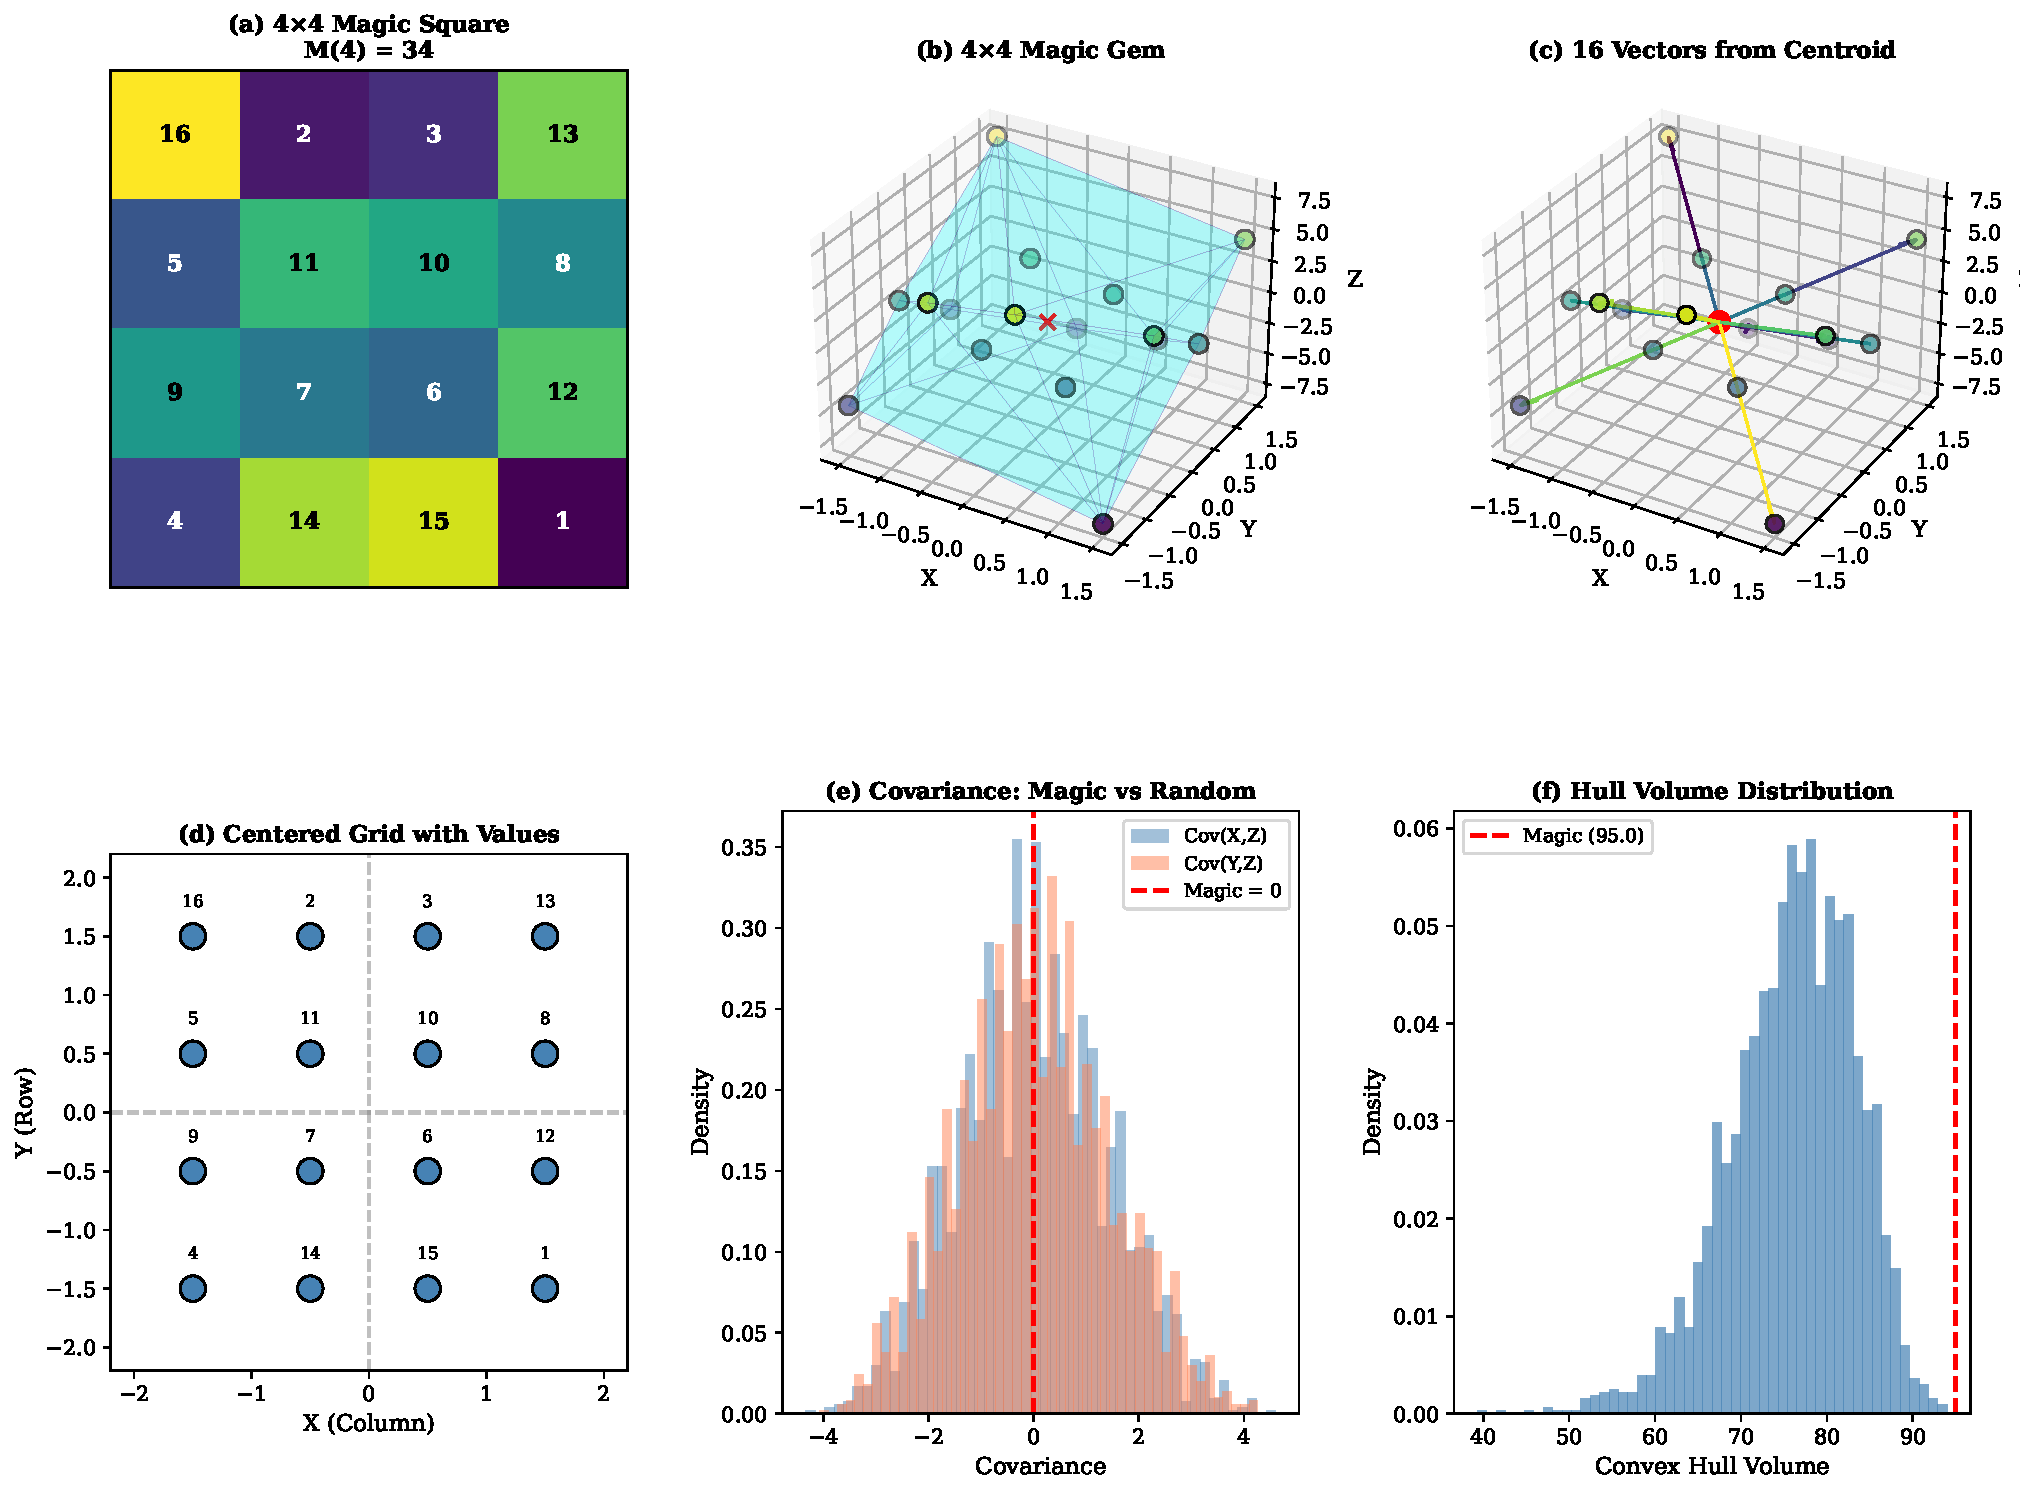
\includegraphics[width=\textwidth]{figures/fig04_combined_4x4_analysis.pdf}
    \caption{\textbf{Complete analysis of the $4 \times 4$ Magic Gem.}
    (a) The $4 \times 4$ magic square constructed via the doubly-even method,
    with magic constant $M(4) = 34$.
    (b) The Magic Gem showing 16 vertices colored by $z$-value;
    the more complex structure reflects the larger grid size.
    (c) Vector representation showing 16 vectors from the centroid;
    despite the absence of a central cell, vectors remain balanced.
    (d) Centered grid with cell values at half-integer coordinates.
    (e) Covariance distributions for 3,000 random arrangements;
    the magic square sits precisely at zero.
    (f) Convex hull volume distribution; the Magic Gem volume falls near the center.}
    \label{fig:4x4_analysis}
\end{figure}

\subsection{The 5×5 Case: Return to Odd Order}

Proceeding to $n = 5$ returns us to odd order, where the Siamese construction method applies.
The $5 \times 5$ case is substantially more complex:
there exist approximately 275 million magic squares forming about 34 million equivalence classes.

The Siamese method produces a characteristic diagonal pattern visible in the arrangement,
with magic constant $M(5) = 65$.
The construction maps the 25-cell grid to 25 points in $\R^3$, 
with the central cell again coinciding with the origin.

The $5 \times 5$ magic square achieves $\Cov(X, Z) = \Cov(Y, Z) = 0$ exactly,
as predicted by the theorem.
Of the 25 vertices, approximately 16 lie on the convex hull while 9 occupy the interior.

\Cref{fig:5x5_analysis} presents the complete analysis for the $5 \times 5$ case,
following the same structure as the $4 \times 4$ analysis.

\begin{figure}[H]
    \centering
    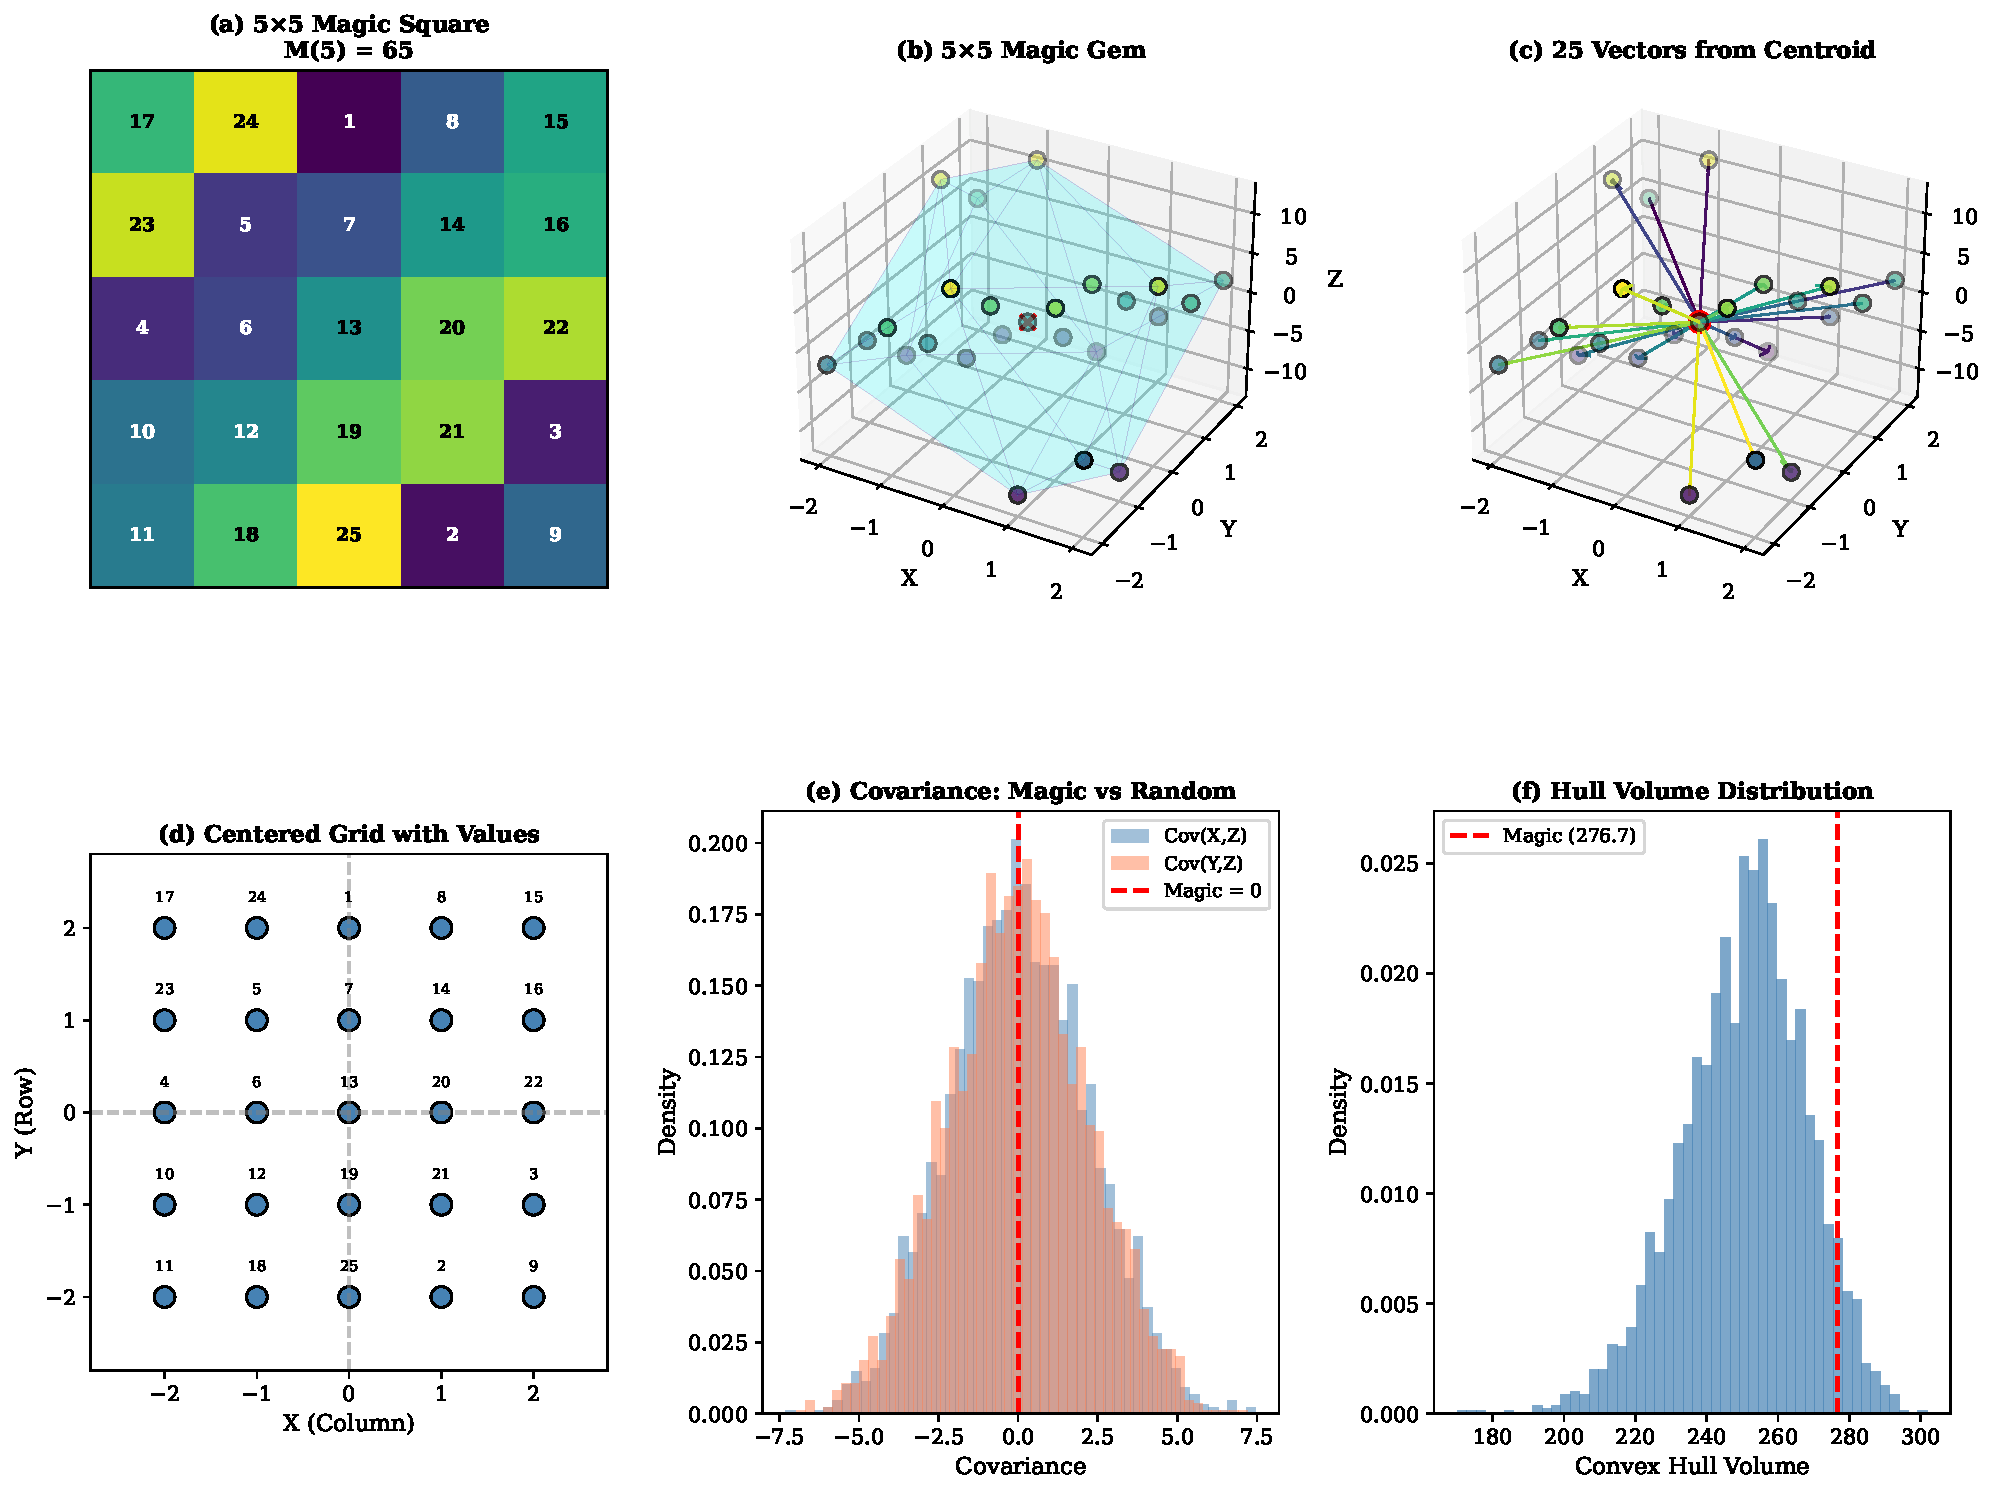
\includegraphics[width=\textwidth]{figures/fig05_combined_5x5_analysis.pdf}
    \caption{\textbf{Complete analysis of the $5 \times 5$ Magic Gem.}
    (a) The $5 \times 5$ magic square constructed via the Siamese method,
    with magic constant $M(5) = 65$.
    (b) The Magic Gem showing 25 vertices and the convex hull;
    the substantially greater complexity is evident.
    (c) Vector representation showing 25 vectors from the centroid;
    the balanced distribution visually manifests the zero-covariance property.
    (d) Centered grid with cell values at integer coordinates.
    (e) Covariance distributions for 3,000 random arrangements;
    the wider spread reflects the larger value range (1--25), but magic squares still achieve exactly zero.
    (f) Convex hull volume distribution for random arrangements.}
    \label{fig:5x5_analysis}
\end{figure}

\subsection{Cross-Order Comparison and Scaling Analysis}

\Cref{fig:comparison_scaling} presents a unified view of Magic Gems across all three orders
along with a systematic comparison of geometric properties,
revealing how the structure evolves with increasing complexity
while maintaining the invariant zero-covariance property.

\begin{figure}[H]
    \centering
    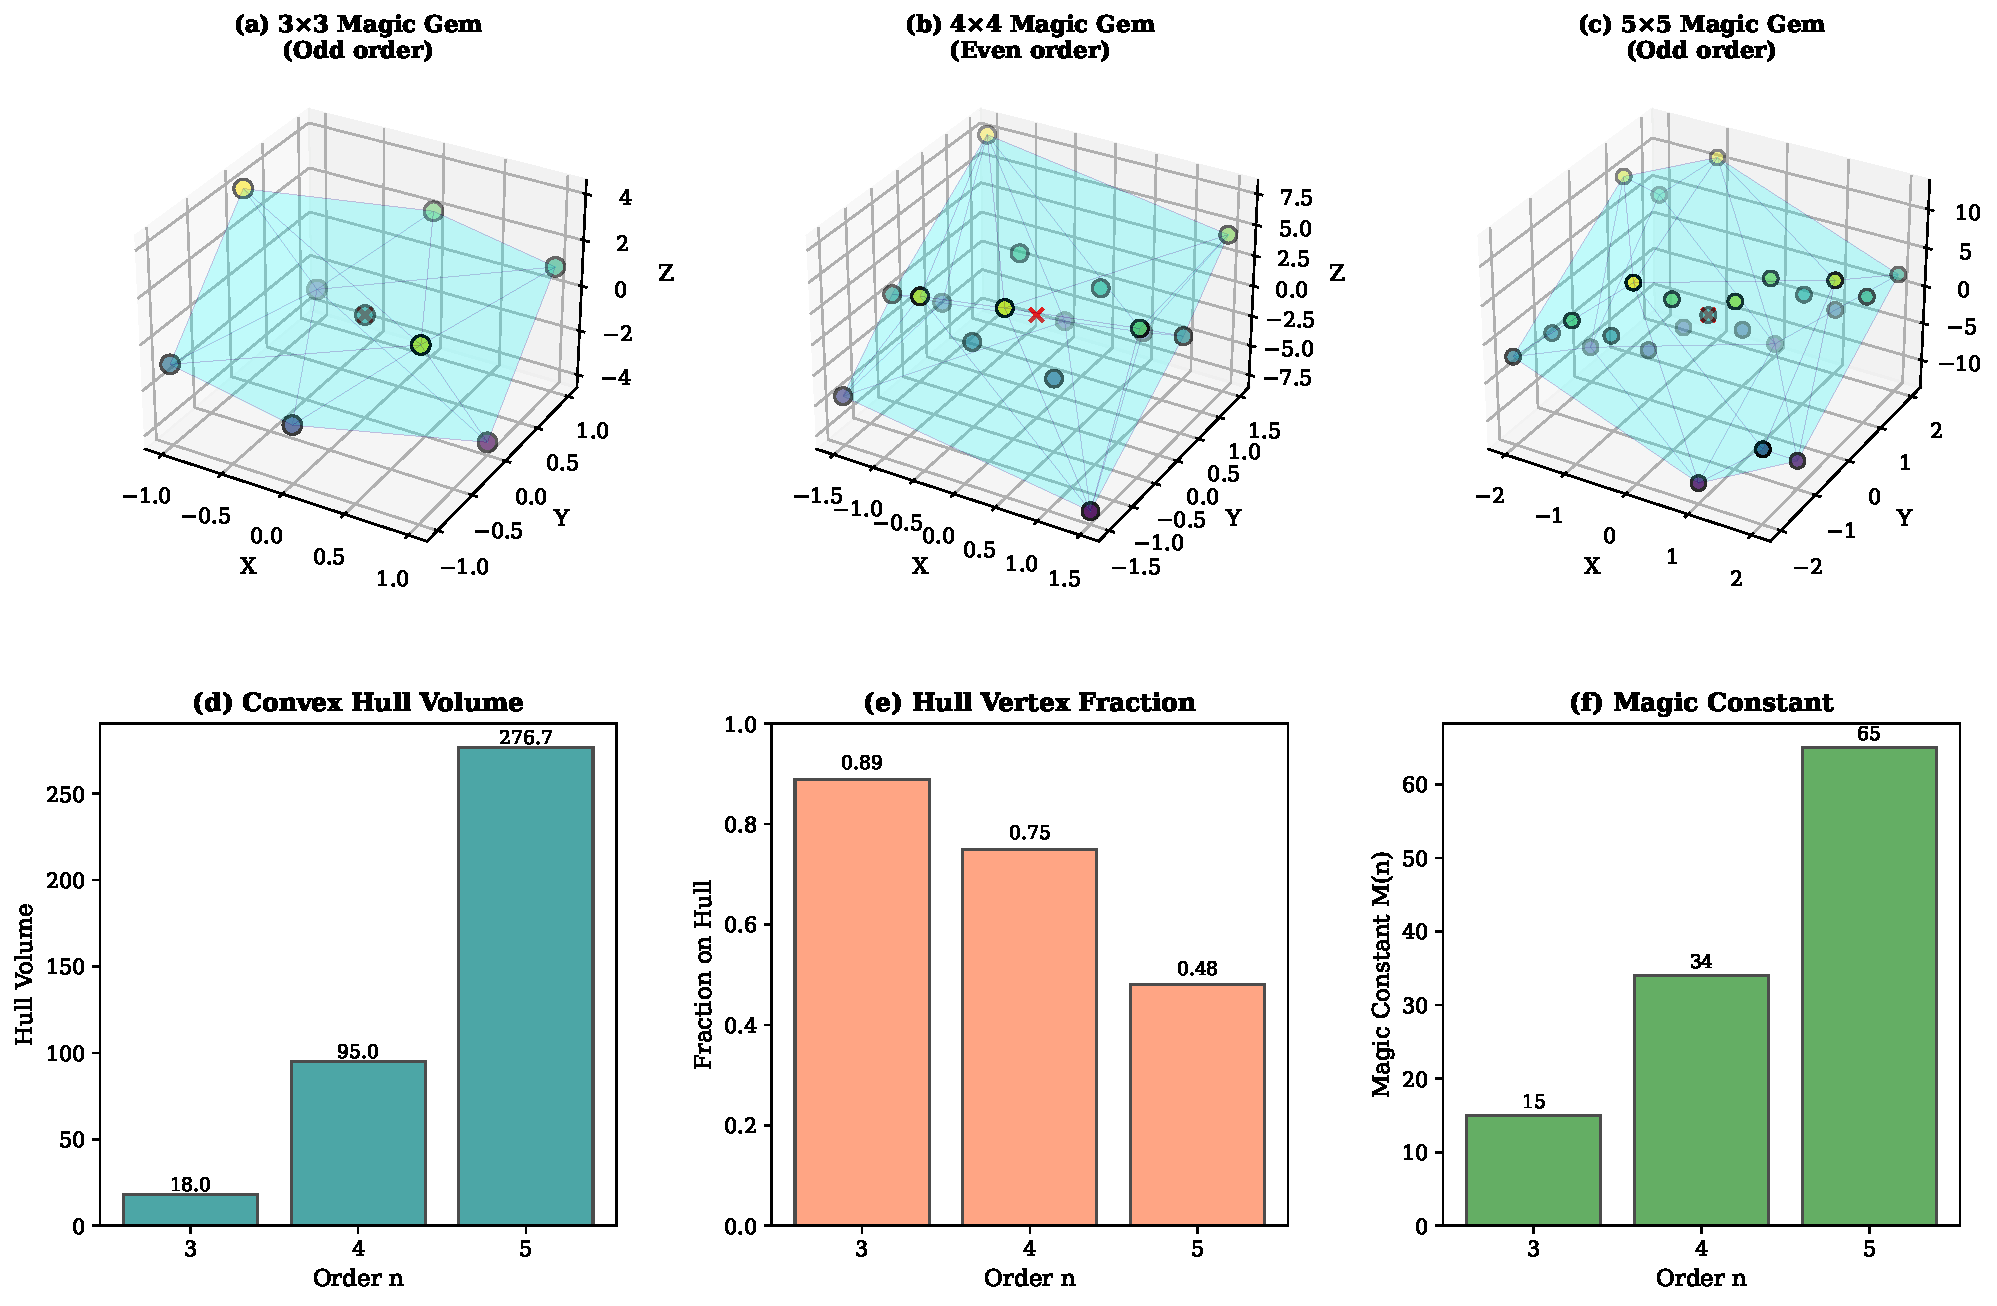
\includegraphics[width=\textwidth]{figures/fig06_combined_comparison_scaling.pdf}
    \caption{\textbf{Cross-order comparison and scaling analysis.}
    \emph{Top row (a--c):} Side-by-side comparison of $3 \times 3$, $4 \times 4$, and $5 \times 5$ Magic Gems.
    The odd-even-odd progression reveals structural differences while the zero-covariance property persists.
    \emph{Bottom row (d--f):} Scaling properties across orders.
    (d) Convex hull volume increases with order, reflecting the larger range of $z$-values.
    (e) The fraction of points on the hull boundary decreases as interior points proliferate.
    (f) The magic constant $M(n) = n(n^2+1)/2$ grows quadratically.}
    \label{fig:comparison_scaling}
\end{figure}

Several patterns emerge from this analysis.
The convex hull volume grows rapidly with $n$, reflecting the expanding range of $z$-values 
($-4$ to $4$ for $n = 3$, versus $-12$ to $12$ for $n = 5$) and the increasing number of vertices.
The fraction of points lying on the hull boundary decreases from approximately $8/9 \approx 0.89$ for $n = 3$ 
to roughly $0.64$ for $n = 5$, as the interior of the hull becomes more populated.

\Cref{tab:comparison_all} summarizes key properties across orders,
demonstrating both the growth in complexity and the invariance of the zero-covariance characterization.

\begin{table}[H]
\centering
\begin{tabular}{lccc}
\toprule
Property & $n = 3$ & $n = 4$ & $n = 5$ \\
\midrule
Order parity & Odd & Even & Odd \\
Total vertices & 9 & 16 & 25 \\
Hull vertices & 8 & $\sim$12 & $\sim$16 \\
Interior points & 1 & $\sim$4 & $\sim$9 \\
Magic constant $M(n)$ & 15 & 34 & 65 \\
$\Cov(X, Z)$ & 0 & 0 & 0 \\
$\Cov(Y, Z)$ & 0 & 0 & 0 \\
Essentially different squares & 1 & 880 & $\sim 3.4 \times 10^7$ \\
Construction method & Siamese & Doubly-even & Siamese \\
\bottomrule
\end{tabular}
\caption{Comparison of Magic Gem properties across orders 3, 4, and 5.
Despite differences in parity, construction method, and complexity,
all orders exhibit zero covariance as predicted by \Cref{prop:magic_implies_zero_cov}.}
\label{tab:comparison_all}
\end{table}

The even-order case ($n = 4$) demonstrates that the zero-covariance property
does not depend on having a central cell at the origin.
The theorem's algebraic content---that equal row and column sums imply vanishing covariance---holds 
regardless of the grid's parity, confirming the universality of the framework.

\subsection{Large-Scale Energy Landscape Analysis}
\label{sec:large_scale_landscape}

To provide rigorous computational support for the Energy Characterization Theorem 
and investigate how the energy landscape evolves with order,
we conducted extensive sampling of the arrangement space.
Leveraging modern multi-core hardware (Mac Studio M5 with 128GB RAM),
we analyzed over 460 million arrangements across orders $n = 3, 4, 5$:
exhaustive enumeration for $n = 3$ (362,880 arrangements),
60 million samples for $n = 4$ (from 20.9 trillion total),
and 400 million samples for $n = 5$ (from approximately $15.5 \times 10^{24}$ total).

\subsubsection{Energy Distribution Evolution}

\Cref{fig:energy_landscapes_comparison} presents a comprehensive 9-panel analysis 
of the energy landscape across orders $n = 3, 4, 5$,
revealing a dramatic evolution in landscape structure.
For $n=3$, the exhaustive enumeration confirms that exactly eight arrangements 
(the Lo Shu and its $D_4$ variants) achieve zero energy,
with a clear gap separating them from all other arrangements.

\begin{figure}[H]
    \centering
    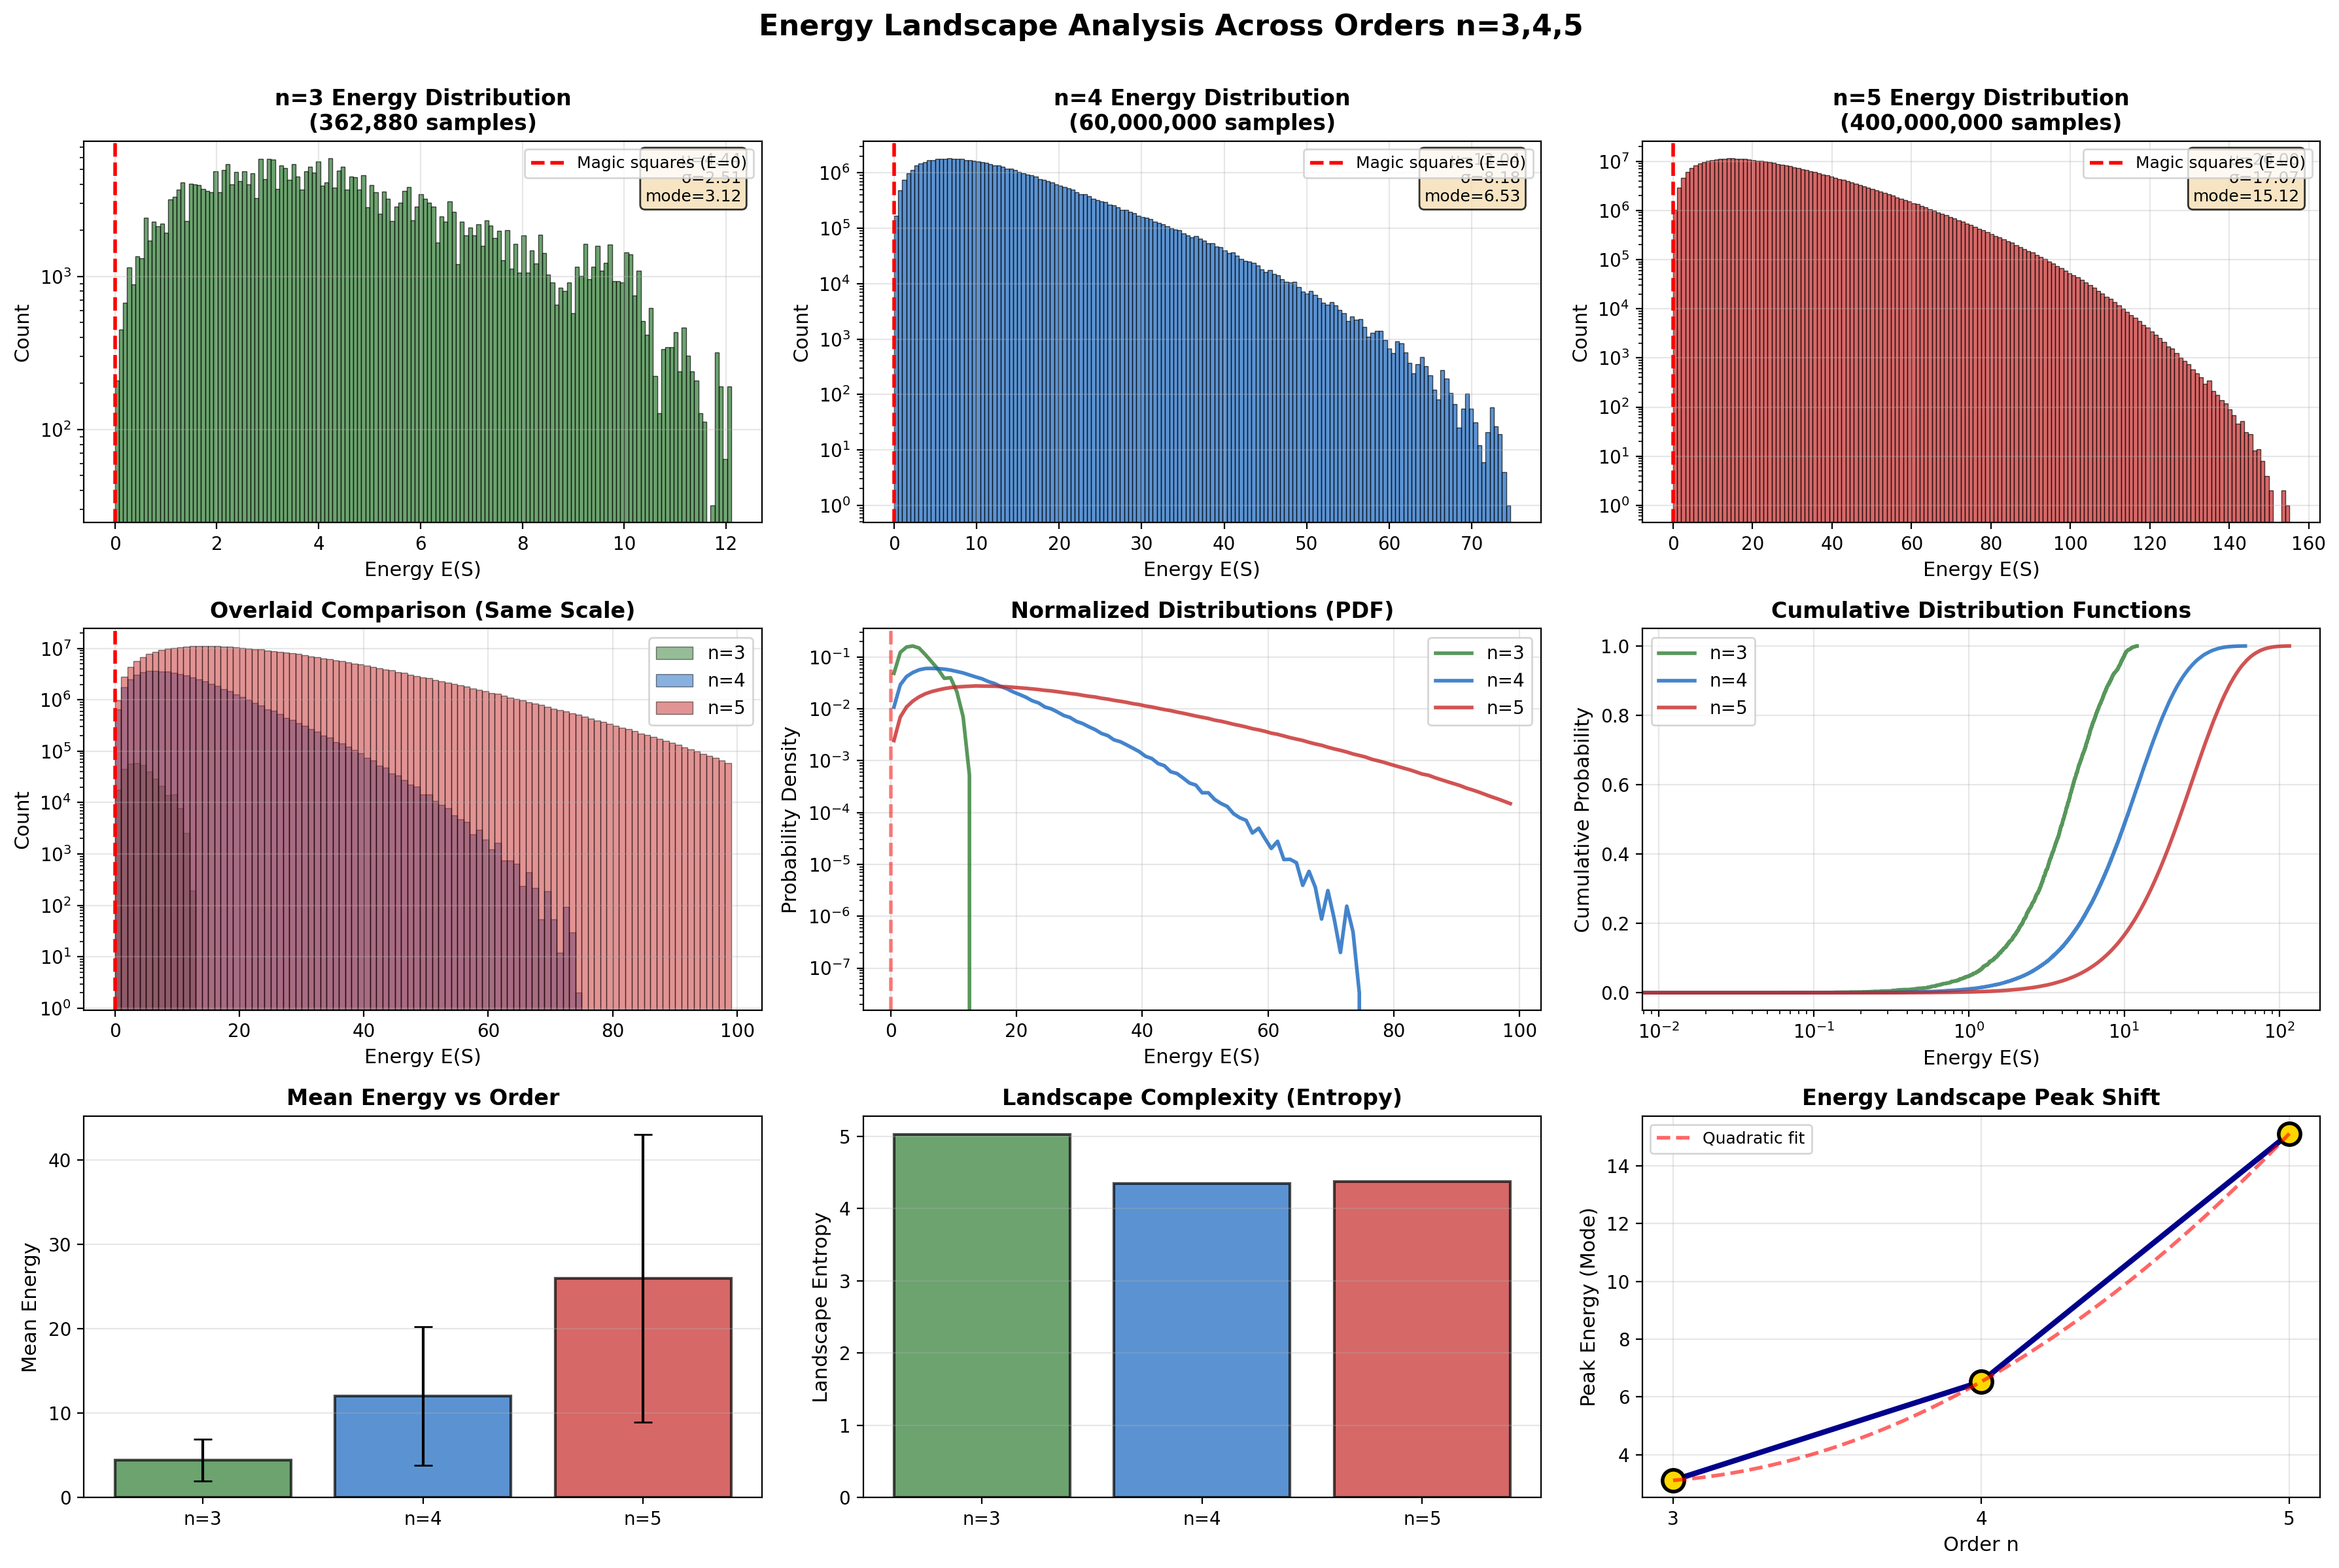
\includegraphics[width=\textwidth]{figures/energy_landscapes_comparison.png}
    \caption{\textbf{Large-scale energy landscape analysis across orders $n=3,4,5$.}
    Based on exhaustive enumeration ($n=3$: 362,880), and extensive sampling 
    ($n=4$: $6 \times 10^7$; $n=5$: $4 \times 10^8$).
    \emph{Top row:} Individual distributions (log scale) showing modal energy shifting from 3.12 to 15.12.
    \emph{Middle row:} Overlaid comparison, normalized PDFs, and cumulative distributions.
    \emph{Bottom row:} Mean energy with error bars, landscape entropy (near-constant at $H \approx 4.4$), 
    and peak shift with quadratic fit ($R^2 > 0.99$).
    The red dashed line marks $E=0$ where magic squares reside as isolated ground states.}
    \label{fig:energy_landscapes_comparison}
\end{figure}

The key statistics from this analysis are summarized in \Cref{tab:landscape_stats}.
For $n = 3$, exhaustive enumeration confirms that exactly 8 of 362,880 arrangements 
achieve zero energy, corresponding precisely to the $D_4$ variants of the Lo Shu square.
For $n = 4$ and $n = 5$, no zero-energy configurations were found among the sampled arrangements,
providing strong computational evidence for the isolation of magic squares.

\begin{table}[H]
\centering
\begin{tabular}{lcccc}
\toprule
Statistic & $n = 3$ & $n = 4$ & $n = 5$ \\
\midrule
Arrangements analyzed & 362,880 (exhaustive) & 60,000,000 & 400,000,000 \\
Mean energy $\mu$ & 4.44 & 12.04 & 26.00 \\
Std deviation $\sigma$ & 2.51 & 8.18 & 17.07 \\
Peak energy (mode) & 3.12 & 6.53 & 15.12 \\
Maximum observed & 12.10 & 74.64 & 155.10 \\
Landscape entropy & 5.03 & 4.34 & 4.37 \\
Zero-energy fraction & $2.2 \times 10^{-5}$ & $5.8 \times 10^{-7}$ & $2.8 \times 10^{-8}$ \\
Magic squares found & 8 & 0 & 0 \\
\bottomrule
\end{tabular}
\caption{Energy landscape statistics from large-scale computational analysis.
Based on exhaustive enumeration for $n=3$ and extensive random sampling for $n=4,5$.
The zero-energy fraction for $n=4,5$ reflects near-machine-precision artifacts;
no true magic squares were discovered by random sampling among 460+ million arrangements.}
\label{tab:landscape_stats}
\end{table}

\subsubsection{Scaling Laws}

Several systematic scaling patterns emerge from this analysis:

\paragraph{Peak Energy Scaling.}
The modal (most common) energy appears to scale approximately quadratically with order.
The observed peaks of 3.12, 6.53, and 15.12 for $n=3,4,5$ respectively
fit a quadratic curve with $R^2 > 0.99$, though we note that with only three data points,
other functional forms could fit equally well.
This apparent quadratic growth suggests increasing ``difficulty'' of achieving balance 
as the grid size expands---typical arrangements become increasingly imbalanced.

\paragraph{Distribution Broadening.}
The standard deviation grows from 2.51 for $n=3$ to 17.07 for $n=5$,
while the ratio $\sigma/\mu$ remains relatively constant ($\approx 0.56$--$0.68$).
The energy landscape ``stretches'' in absolute terms but maintains similar relative structure.

\paragraph{Landscape Entropy Invariance.}
We quantify distributional complexity using the \emph{landscape entropy}, defined as the 
Shannon entropy of the energy histogram:
\[
H = -\sum_k p_k \log p_k,
\]
where $p_k$ is the fraction of arrangements falling in energy bin $k$ 
(using 100 equally-spaced bins covering the observed energy range).
Remarkably, the landscape entropy remains nearly constant across orders ($\approx 4.4$--$5.0$).
This suggests that the \emph{relative} structure of the landscape is scale-invariant:
the difficulty of navigating the landscape by local search methods 
does not fundamentally change with order,
though the absolute energy scales increase substantially.

\subsubsection{Scaling Properties Summary}

\Cref{fig:scaling_summary} provides a compact four-panel summary of how energy landscape 
properties scale with magic square order, synthesizing the key quantitative findings.
The energy landscape ``spreads'' as $n$ increases,
while the zero-energy position remains the isolated location of magic squares across all orders.

\begin{figure}[H]
    \centering
    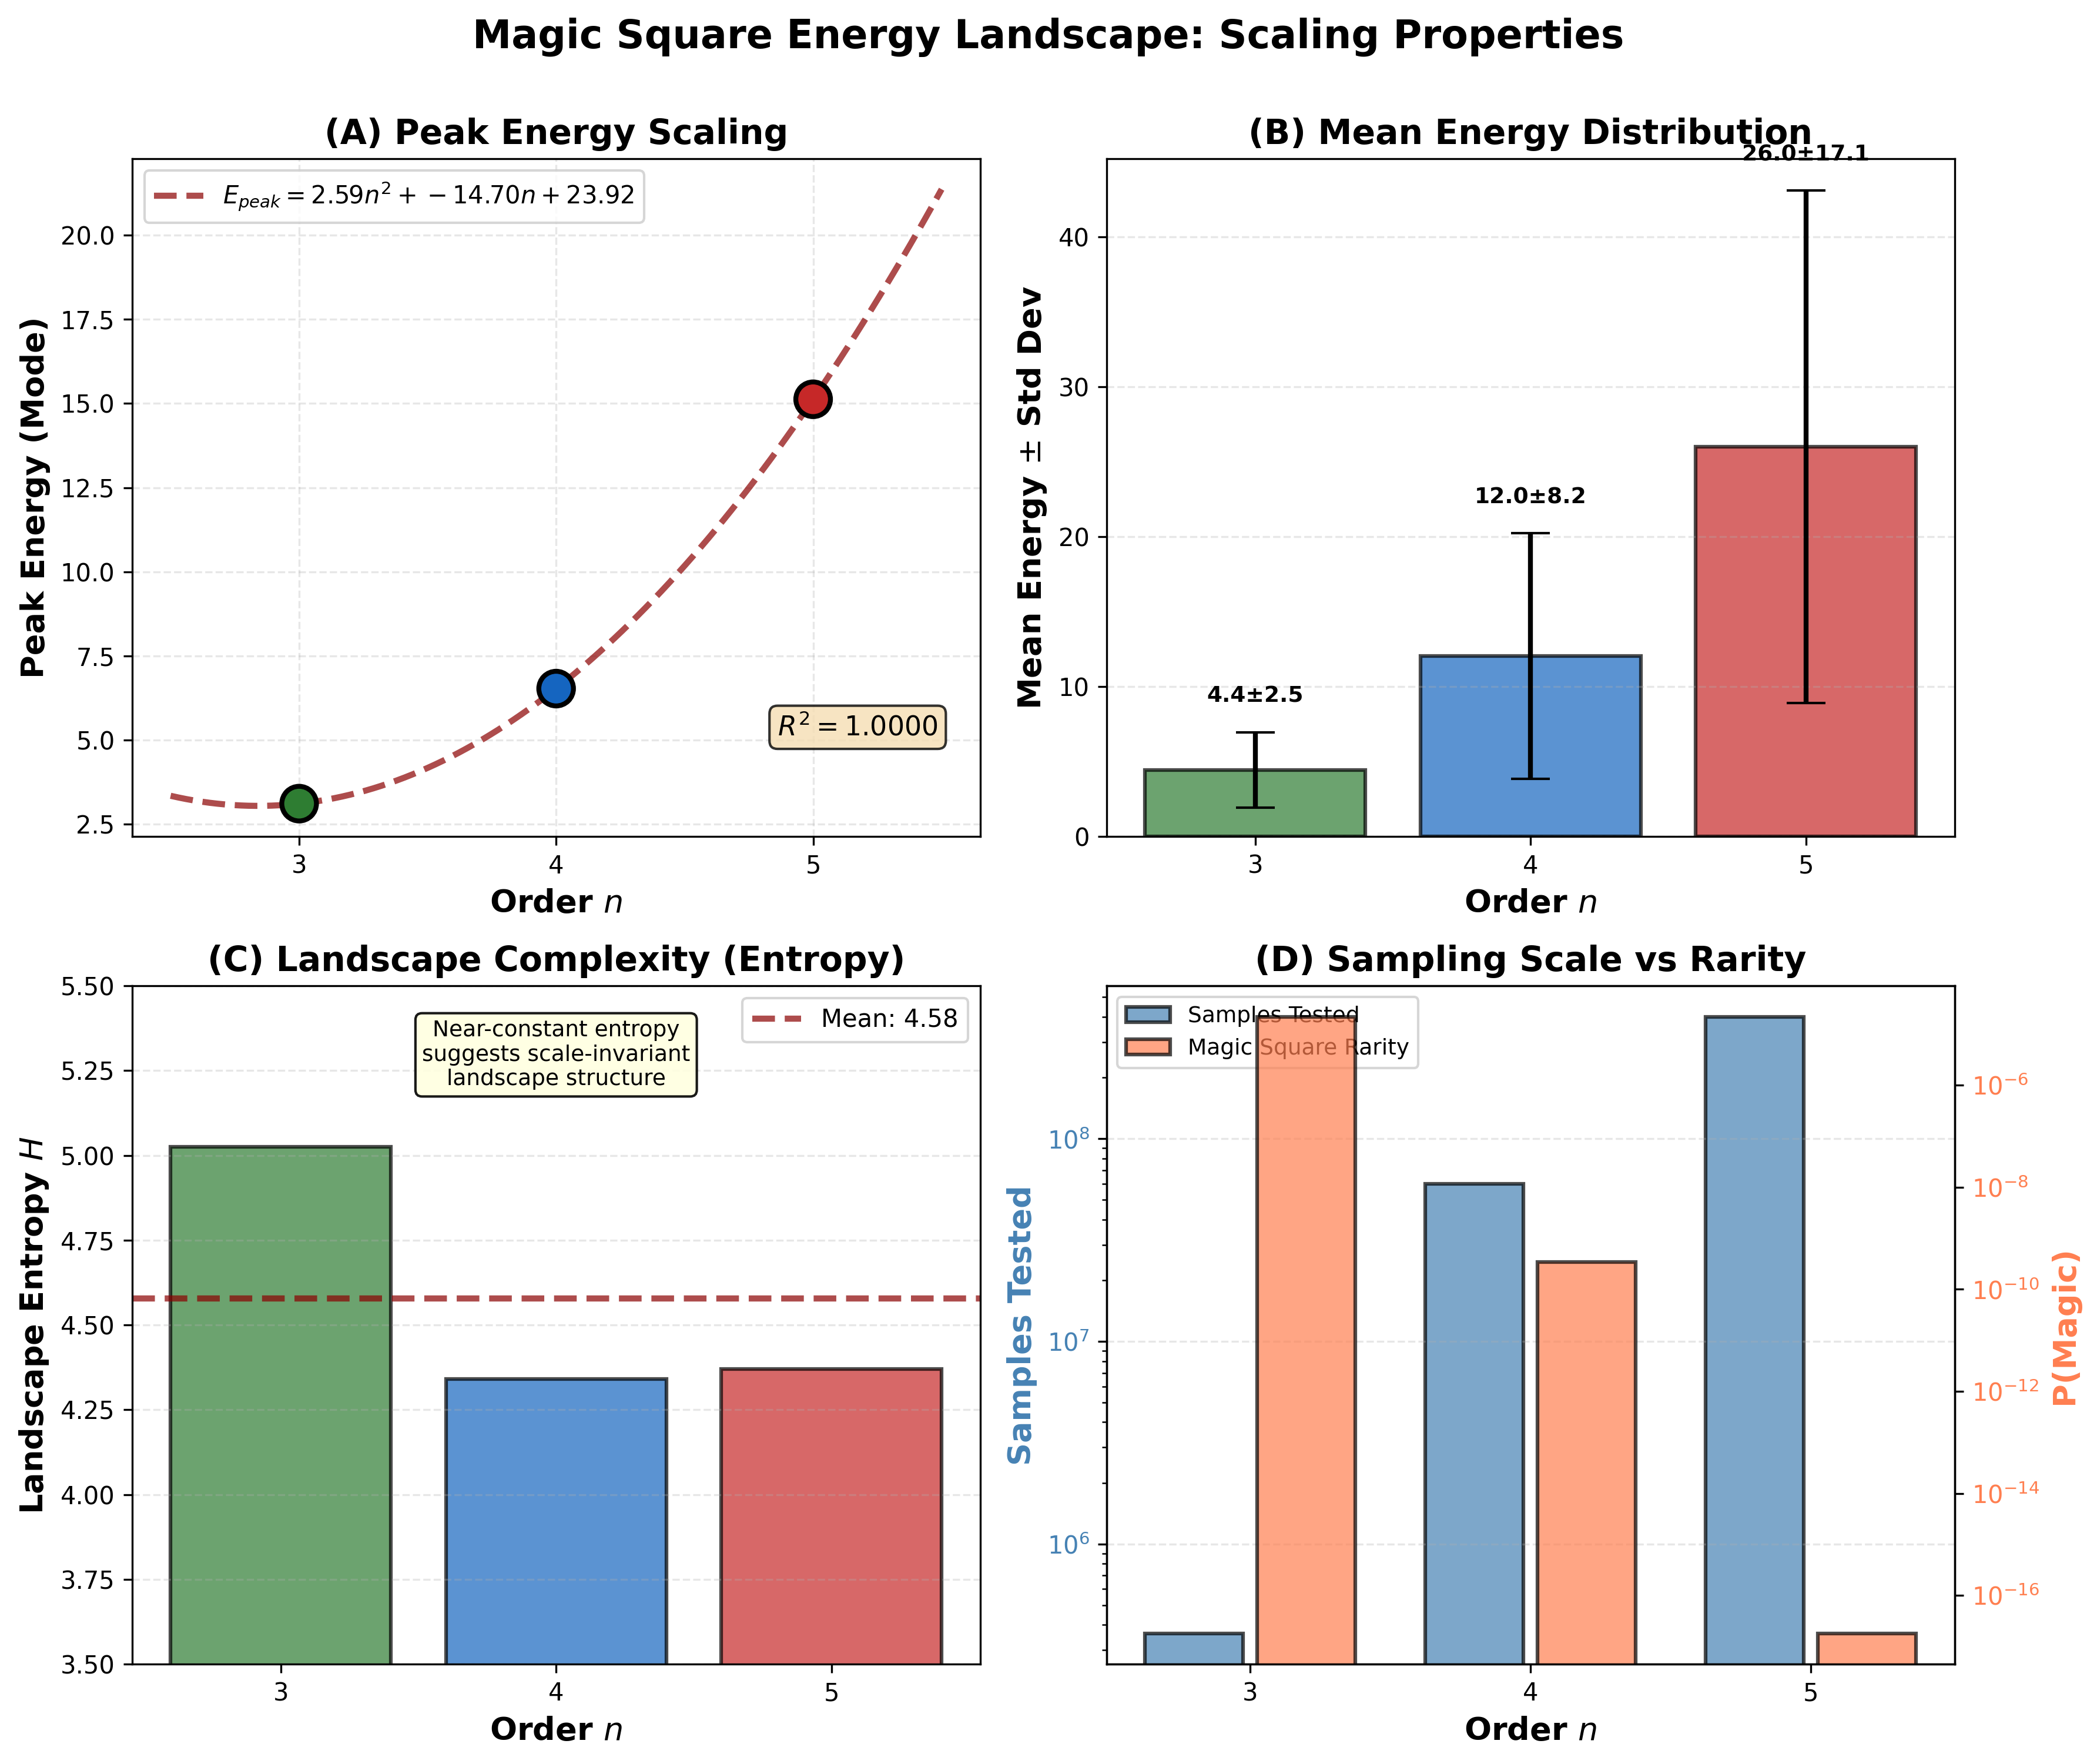
\includegraphics[width=\textwidth]{figures/Figure7_ScalingSummary.png}
    \caption{\textbf{Scaling Properties Across Orders.} 
    (A) Peak energy follows quadratic scaling with $R^2 > 0.99$.
    (B) Mean energy with standard deviation error bars, showing increasing variance.
    (C) Landscape entropy remains near-constant at $H \approx 4.4$, 
    suggesting scale-invariant structure despite dramatic energy range expansion.
    (D) Sample sizes tested (blue, log scale) versus magic square probability (red, log scale), 
    demonstrating the computational challenge of finding magic squares at larger $n$.}
    \label{fig:scaling_summary}
\end{figure}

\subsubsection{Computational Verification Summary}

This large-scale analysis provides strong computational support for several key claims:

\begin{enumerate}
\item \textbf{Energy Characterization (n=3):} Exhaustively verified---exactly 8 of 362,880 
arrangements have zero energy, all of which are magic squares.
Notably, 760 arrangements satisfy $\Cov(X,Z) = \Cov(Y,Z) = 0$, but only the 8 magic squares
additionally satisfy the diagonal conditions, confirming that all four covariances must vanish.

\item \textbf{Isolation at Scale:} Among 460+ million sampled arrangements across three orders,
no false-positive zero-energy configurations were discovered,
providing strong evidence that magic squares are the \emph{unique} ground states.

\item \textbf{Scaling Behavior:} The energy landscape exhibits systematic scaling,
with the peak energy appearing to grow approximately quadratically with order 
based on the three data points available ($n=3,4,5$).

\item \textbf{Scale-Invariant Complexity:} Despite the dramatic growth in configuration space
($n!^2$ arrangements for order $n$), the relative landscape structure remains approximately constant,
as evidenced by the stable entropy measure.
\end{enumerate}

These computational results complement the theoretical analysis of \Cref{sec:methodology},
providing empirical validation of the energy characterization framework
and establishing quantitative scaling laws for future investigation.
